\documentclass{article}
\usepackage{graphicx} % Required for inserting images
\usepackage[utf8]{inputenc}
\usepackage{longtable}
\usepackage{tabu}
\usepackage{amsmath}
\usepackage{float}
\usepackage{pdfpages}
\usepackage[main=greek,english]{babel}
\newcommand\tab[1][1cm]{\hspace*{#1}}
\newcommand \en {\selectlanguage{english}}
\newcommand \gr {\selectlanguage{greek}}


\begin{document}

\gr
\section{Εγχειρίδιο χρήσης κώδικα}
Μαζί με τον κώδικα και τα γραφήματα, δημιουργείται για κάθε καταγραφή μία αναφορά προς το γιατρό ή γενικότερα τον υπεύθυνο ιατρικό ερευνητή. Η αναφορά αυτή περιέχει τις μέγιστες τιμές κάθε μετρικής και μεθόδου, τη μέση τιμή τους και τη μέση τιμή κάθε μετρικής και μεθόδου των ασθενών της πρώτης φάσης του έργου προς
σύγκριση. Επιπλέον εμφανίζεται στην  αναφορά και το γράφημα που έχει παραχθεί. Στη συνέχεια παρουσιάζεται το τελικό γράφημα με τις περιοχές που εκτιμώνται ως επικίνδυνες (σε κάθε περίπτωση παρουσιάζεται διαφορετική μετρική, ανάλογα με την εγκυρότητά τους). Στις επόμενες σελίδες φαίνεται η αναφορά, όπως ακριβώς παράγεται για τον εκάστοτε ειδικό.
\par
Τα βήματα της παραγωγής της αναφοράς παράγονται ως εξής: 
\begin{itemize}
    \item Στο τερματικό, δίνονται ως παράμετροι το όνομα της βιβλιοθήκης, μια μεταβλητή που αντιστοιχεί στο αν θα παραχθούν τα κυματίδια \en Haar \gr και ο τύπος πειραμάτων στην περίπτωση που πρόκειται για κάποια από τος βιβλιοθήκες που περιέχουν φυσιολογικό σήμα.
    \item Κατά την εκτέλεση αυτής της εντολής, παράγεται για κάθε καταγραφή το γράφημα και το αρχείο με τις μέγιστες και τις μέσες τιμές των μετρικών.
    \item Για να παραχθεί η τελική αναφορά, το παραγόμενο αρχείο πρέπει να ενσωματωθεί στο αρχείο της αναφοράς (το παραγόμενο αρχείο περιέχει μόνο τις τιμές, ενω το βασικό αρχείο περιέχει τους πίνακες στους οποίους θα περαστούν οι τιμές).   
\end{itemize}
Παρακάτω παρουσιάζεται ένα δείγμα της τελικής αναφοράς, όπως αυτή θα παραδοθεί με σκοπό να μελετηθεί η εγκυρότητά της. 
\par
\textbf{Σημείωση}: Η προσθήκη νέων μετρικών ή γραφημάτων είναι αρκετά εύκολη, καθώς απλώς προσθέτεται στον αρχικό κώδικα (ή αφαιρείται από αυτόν) ο υπολογισμός τους και στη συνέχεια παράγεται για κάθε ασθενή της βάσης δεδομένων αυτόματα η μέση και η μέγιστη τιμή. Το μέγεθος παραθύρου δε χρειάζεται να τεθεί ως παράμετρος κατά την εκτέλεση του κώδικα, καθώς υπολογίζεται αυτόματα μέσα από ένα αρχικό πλήθος μεγεθών. 

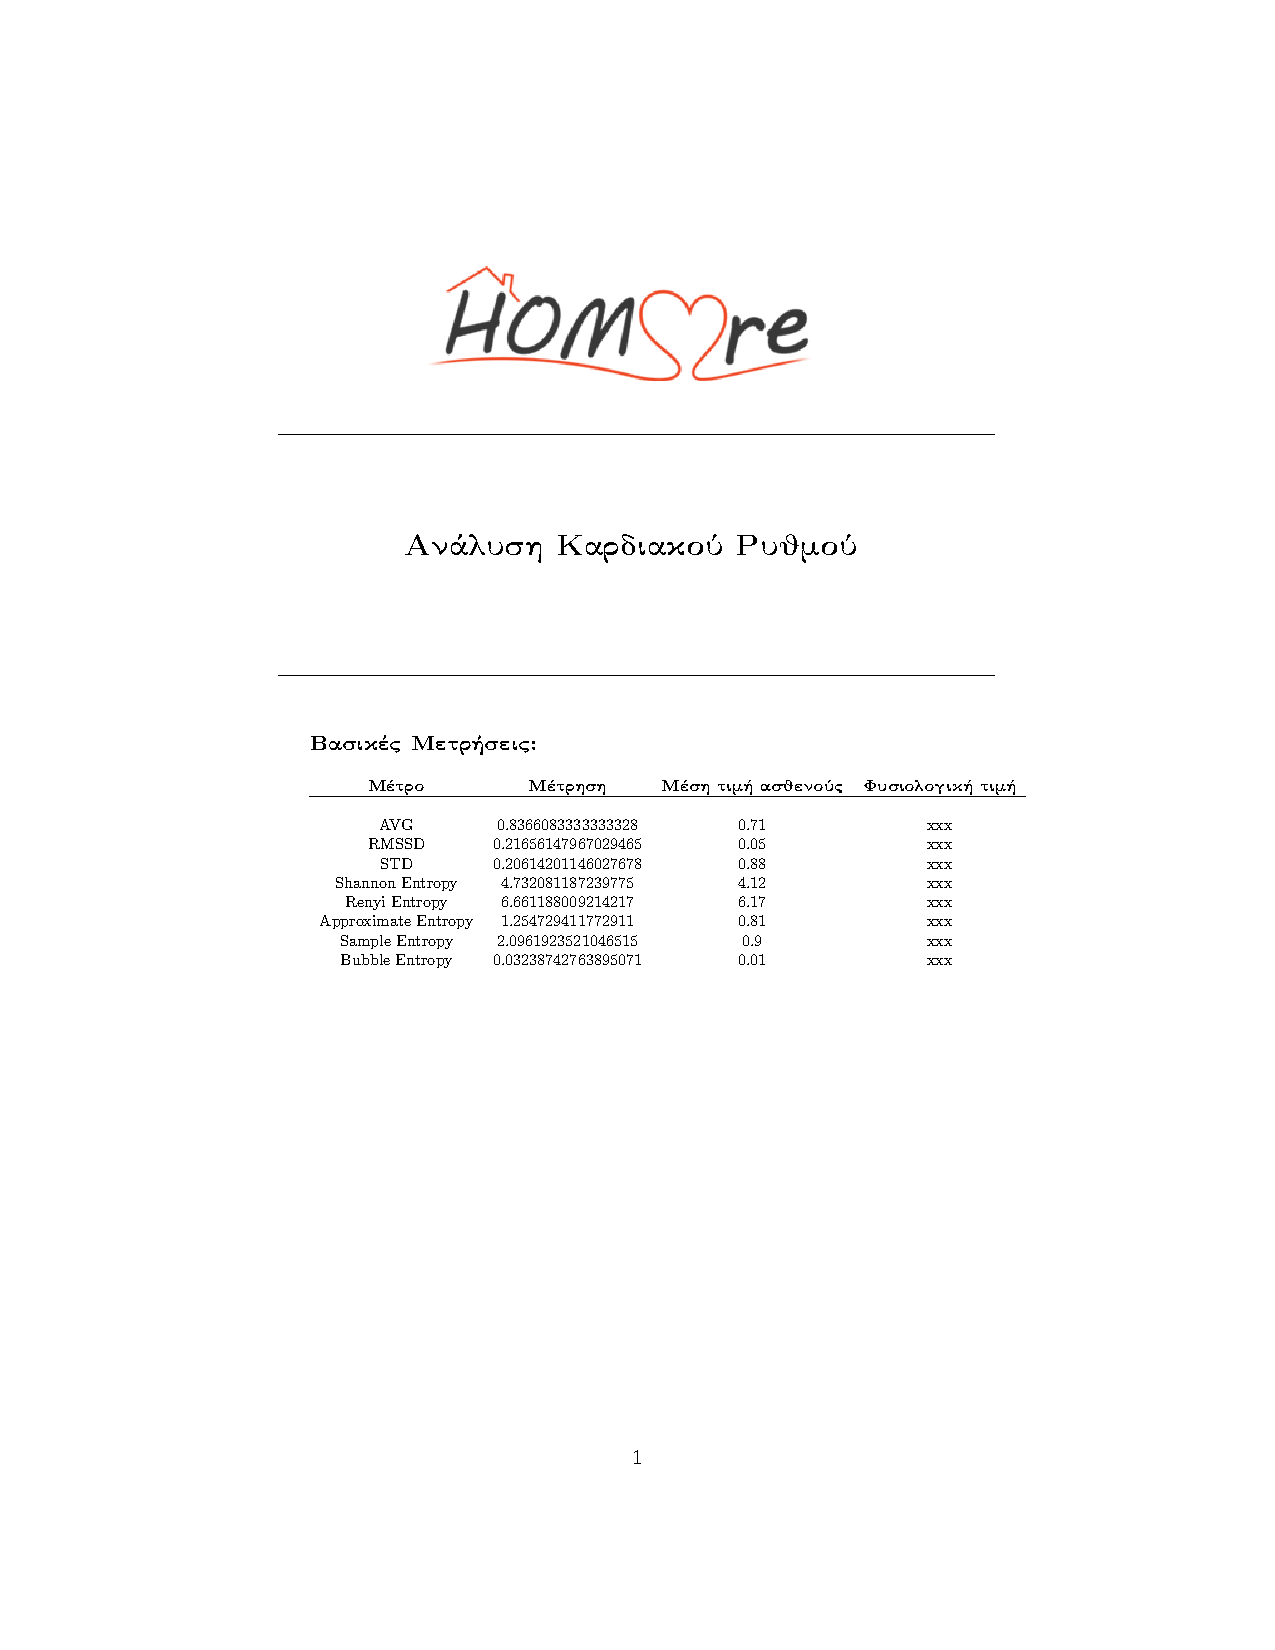
\includepdf[page={1, 2, 3}]{Report.pdf}
\end{document}
